% GNUPLOT: LaTeX picture with Postscript
\begingroup
  \makeatletter
  \providecommand\color[2][]{%
    \GenericError{(gnuplot) \space\space\space\@spaces}{%
      Package color not loaded in conjunction with
      terminal option `colourtext'%
    }{See the gnuplot documentation for explanation.%
    }{Either use 'blacktext' in gnuplot or load the package
      color.sty in LaTeX.}%
    \renewcommand\color[2][]{}%
  }%
  \providecommand\includegraphics[2][]{%
    \GenericError{(gnuplot) \space\space\space\@spaces}{%
      Package graphicx or graphics not loaded%
    }{See the gnuplot documentation for explanation.%
    }{The gnuplot epslatex terminal needs graphicx.sty or graphics.sty.}%
    \renewcommand\includegraphics[2][]{}%
  }%
  \providecommand\rotatebox[2]{#2}%
  \@ifundefined{ifGPcolor}{%
    \newif\ifGPcolor
    \GPcolorfalse
  }{}%
  \@ifundefined{ifGPblacktext}{%
    \newif\ifGPblacktext
    \GPblacktexttrue
  }{}%
  % define a \g@addto@macro without @ in the name:
  \let\gplgaddtomacro\g@addto@macro
  % define empty templates for all commands taking text:
  \gdef\gplbacktext{}%
  \gdef\gplfronttext{}%
  \makeatother
  \ifGPblacktext
    % no textcolor at all
    \def\colorrgb#1{}%
    \def\colorgray#1{}%
  \else
    % gray or color?
    \ifGPcolor
      \def\colorrgb#1{\color[rgb]{#1}}%
      \def\colorgray#1{\color[gray]{#1}}%
      \expandafter\def\csname LTw\endcsname{\color{white}}%
      \expandafter\def\csname LTb\endcsname{\color{black}}%
      \expandafter\def\csname LTa\endcsname{\color{black}}%
      \expandafter\def\csname LT0\endcsname{\color[rgb]{1,0,0}}%
      \expandafter\def\csname LT1\endcsname{\color[rgb]{0,1,0}}%
      \expandafter\def\csname LT2\endcsname{\color[rgb]{0,0,1}}%
      \expandafter\def\csname LT3\endcsname{\color[rgb]{1,0,1}}%
      \expandafter\def\csname LT4\endcsname{\color[rgb]{0,1,1}}%
      \expandafter\def\csname LT5\endcsname{\color[rgb]{1,1,0}}%
      \expandafter\def\csname LT6\endcsname{\color[rgb]{0,0,0}}%
      \expandafter\def\csname LT7\endcsname{\color[rgb]{1,0.3,0}}%
      \expandafter\def\csname LT8\endcsname{\color[rgb]{0.5,0.5,0.5}}%
    \else
      % gray
      \def\colorrgb#1{\color{black}}%
      \def\colorgray#1{\color[gray]{#1}}%
      \expandafter\def\csname LTw\endcsname{\color{white}}%
      \expandafter\def\csname LTb\endcsname{\color{black}}%
      \expandafter\def\csname LTa\endcsname{\color{black}}%
      \expandafter\def\csname LT0\endcsname{\color{black}}%
      \expandafter\def\csname LT1\endcsname{\color{black}}%
      \expandafter\def\csname LT2\endcsname{\color{black}}%
      \expandafter\def\csname LT3\endcsname{\color{black}}%
      \expandafter\def\csname LT4\endcsname{\color{black}}%
      \expandafter\def\csname LT5\endcsname{\color{black}}%
      \expandafter\def\csname LT6\endcsname{\color{black}}%
      \expandafter\def\csname LT7\endcsname{\color{black}}%
      \expandafter\def\csname LT8\endcsname{\color{black}}%
    \fi
  \fi
  \setlength{\unitlength}{0.0500bp}%
  \begin{picture}(15840.00,5040.00)%
    \gplgaddtomacro\gplbacktext{%
    }%
    \gplgaddtomacro\gplfronttext{%
      \csname LTb\endcsname%
      \put(0,-124){\makebox(0,0){\centering\scriptsize$\mathsf{2}$}}%
      \put(1440,-124){\makebox(0,0){\centering\scriptsize$\mathsf{0.000}$}}%
      \put(2879,-124){\makebox(0,0){\centering\scriptsize$\mathsf{0.000}$}}%
      \put(4319,-124){\makebox(0,0){\centering\scriptsize$\mathsf{0.000}$}}%
      \put(5759,-124){\makebox(0,0){\centering\scriptsize$\mathsf{0.000}$}}%
      \put(7199,-124){\makebox(0,0){\centering\scriptsize$\mathsf{1}$}}%
      \put(8638,-124){\makebox(0,0){\centering\scriptsize\textsf{Gain}}}%
      \put(10078,-124){\makebox(0,0){\centering\scriptsize$\mathsf{0.000}$}}%
      \put(11518,-124){\makebox(0,0){\centering\scriptsize\textsf{Unused}}}%
      \put(12958,-124){\makebox(0,0){\centering\scriptsize$\mathsf{0.000}$}}%
      \put(14397,-124){\makebox(0,0){\centering\scriptsize$\mathsf{2.857}$}}%
      \put(15837,-124){\makebox(0,0){\centering\scriptsize$\mathsf{1.000}$}}%
      \put(11784,458){\makebox(0,0){\centering\scriptsize $\mathsf{\phantom{0\;00}0.000}$}}%
      \put(0,5165){\makebox(0,0){\centering\scriptsize$\mathsf{20}$}}%
      \put(1440,5165){\makebox(0,0){\centering\scriptsize$\mathsf{10.000}$}}%
      \put(2879,5165){\makebox(0,0){\centering\scriptsize$\mathsf{1\;500.000}$}}%
      \put(4319,5165){\makebox(0,0){\centering\scriptsize$\mathsf{20.000}$}}%
      \put(5759,5165){\makebox(0,0){\centering\scriptsize$\mathsf{100.000}$}}%
      \put(7199,5165){\makebox(0,0){\centering\scriptsize$\mathsf{400}$}}%
      \put(8638,5165){\makebox(0,0){\centering\scriptsize\textsf{Gain Ratio}}}%
      \put(10078,5165){\makebox(0,0){\centering\scriptsize$\mathsf{100.000}$}}%
      \put(11518,5165){\makebox(0,0){\centering\scriptsize$\mathsf{100.000}$}}%
      \put(12958,5165){\makebox(0,0){\centering\scriptsize$\mathsf{10\;000.000}$}}%
      \put(14397,5165){\makebox(0,0){\centering\scriptsize$\mathsf{53.333}$}}%
      \put(15837,5165){\makebox(0,0){\centering\scriptsize$\mathsf{21.600}$}}%
      \put(0,5442){\makebox(0,0){\centering\small\textsf{\phantom{p}}$K$ \textsf{and} $J$\textsf{\phantom{p}}}}%
      \put(1440,5442){\makebox(0,0){\centering\small\textsf{\phantom{p}}$\eta(0)$\textsf{\phantom{p}}}}%
      \put(2879,5442){\makebox(0,0){\centering\small\textsf{\phantom{p}}$\tau_{1}$\textsf{\phantom{p}}}}%
      \put(4319,5442){\makebox(0,0){\centering\small\textsf{\phantom{p}}$\sigma(0)$\textsf{\phantom{p}}}}%
      \put(5759,5442){\makebox(0,0){\centering\small\textsf{\phantom{p}}$\tau_{2}$\textsf{\phantom{p}}}}%
      \put(7199,5659){\makebox(0,0){\centering\small\textsf{\phantom{p}Minimum\phantom{p}}}}%
      \put(7199,5442){\makebox(0,0){\centering\small\textsf{\phantom{p}examples\phantom{p}}}}%
      \put(8638,5659){\makebox(0,0){\centering\small\textsf{\phantom{p}Test\phantom{p}}}}%
      \put(8638,5442){\makebox(0,0){\centering\small\textsf{\phantom{p}heuristic\phantom{p}}}}%
      \put(10078,5659){\makebox(0,0){\centering\small\textsf{\phantom{p}Pessimistic\phantom{p}}}}%
      \put(10078,5442){\makebox(0,0){\centering\small\textsf{\phantom{p}confidence\phantom{p}}}}%
      \put(11518,5659){\makebox(0,0){\centering\small\textsf{\phantom{p}Fisher's\phantom{p}}}}%
      \put(11518,5442){\makebox(0,0){\centering\small\textsf{\phantom{p}confidence\phantom{p}}}}%
      \put(12958,5659){\makebox(0,0){\centering\small\textsf{\phantom{p}Attribute\phantom{p}}}}%
      \put(12958,5442){\makebox(0,0){\centering\small\textsf{\phantom{p}redundancy\phantom{p}}}}%
      \put(14397,5442){\makebox(0,0){\centering\small\textsf{\phantom{p}}${\cal E}_{G}$\textsf{\phantom{p}}}}%
      \put(15837,5442){\makebox(0,0){\centering\small\textsf{\phantom{p}}${\cal E}_{C}$\textsf{\phantom{p}}}}%
      \put(-355,3919){\makebox(0,0){\scriptsize $\mathsf{\phantom{0\;0000.}16}$}}%
      \put(1083,79){\makebox(0,0){\scriptsize $\mathsf{\phantom{0\;00}0.156}$}}%
      \put(2522,4838){\makebox(0,0){\scriptsize $\mathsf{1\;429.688}$}}%
      \put(3962,3172){\makebox(0,0){\scriptsize $\mathsf{\phantom{0\;0}12.750}$}}%
      \put(5402,4563){\makebox(0,0){\scriptsize $\mathsf{\phantom{0\;0}89.063}$}}%
      \put(6842,488){\makebox(0,0){\scriptsize $\mathsf{\phantom{0\;0000.}44}$}}%
      \put(9721,2176){\makebox(0,0){\scriptsize $\mathsf{\phantom{0\;0}42.188}$}}%
      \put(12600,4041){\makebox(0,0){\scriptsize $\mathsf{7\;968.750}$}}%
      \put(14040,1576){\makebox(0,0){\scriptsize $\mathsf{\phantom{0\;0}19.048}$}}%
      \put(15480,430){\makebox(0,0){\scriptsize $\mathsf{\phantom{0\;00}3.067}$}}%
    }%
    \gplbacktext
    \put(0,0){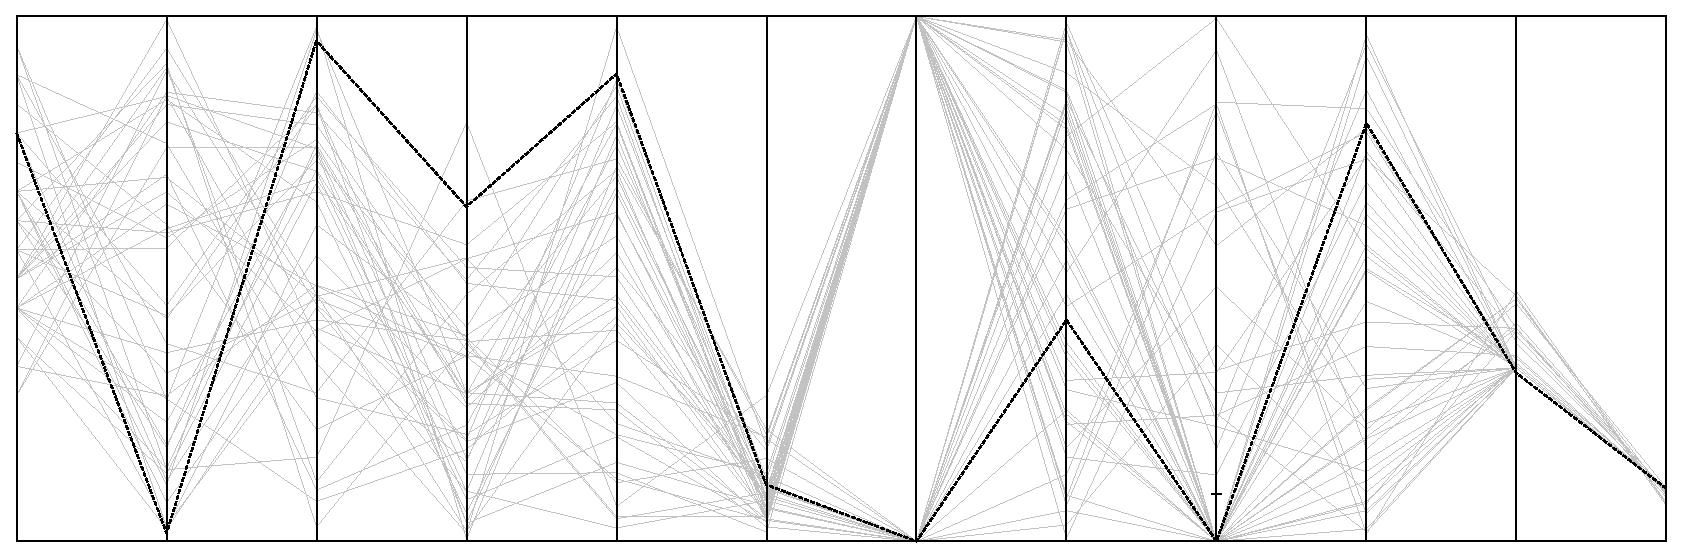
\includegraphics{hybridSOM-c4-5_monks3_gnuplot_conditions}}%
    \gplfronttext
  \end{picture}%
\endgroup
